\section{Prevenzione e gestione delle emergenze sanitarie}

\subsection{Introduzione}

Cosa intendiamo per emergenze sanitarie? ``Definiamo emergenze quelle
situazioni in cui è prevista una gestione che va al di là di ciò che
accade routinariamente''.

Alcuni esempi possono essere: attentati, pandemie, terremoti o le
problematiche legate alla gestione in acuto della popolazione migrante.
Il focus in ambito sanitario è sempre puntato su quella che è la
gestione delle problematiche sanitarie legate all'emergenza.

\emph{Definizione classica:} evento straordinario che si ritiene possa
costituire un rischio significativo per la salute della popolazione e
richiedere potenzialmente una risposta coordinata per minimizzare il
rischio ed il pericolo per la salute pubblica.

Glossario WHO da cui è tratta la definizione, utile per approfondimenti.

\begin{figure}[!ht]
\centering
	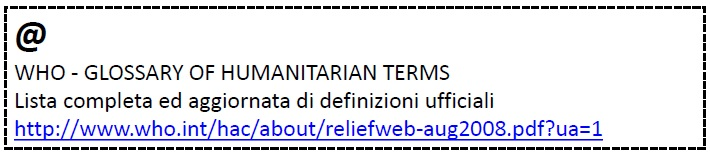
\includegraphics[width=0.5\textwidth]{26/image1.jpeg}
	\end{figure}

Legato al concetto di emergenza è il concetto di
\emph{\textbf{``}preparedness\textbf{''}}.

Questo termine, difficilmente traducibile, può essere spiegato con un
esempio: quando si verifica un terremoto, ci deve essere dietro un
sistema che si attivi, una volta dichiarato lo stato di emergenza, per
gestire le problematiche sanitarie.

Il concetto di \emph{preparedness} riguarda quindi la capacità e la
conoscenza, a vari livelli (es. dei governi, delle organizzazioni, delle
comunità e dei singoli individui) di anticipare e di prevenire ma anche
di rispondere in maniera efficace all'impatto di possibili emergenze.

Un ulteriore concetto, approfondito dalla Comunità Europea, è il
\emph{``cross-border threaths to health''}, ossia minacce per la sanità
che sono definite cross-border, ovvero che non mantengono i confini
nazionali. Sono quindi dei rischi che possono essere di origine
biologica, chimica, ambientale o sconosciuta, che possono manifestarsi
ed avere un impatto sovranazionale, comunitario. Per cui esistono una
serie di meccanismi di risposta non solo nazionali ma sovranazionali (in
questo caso europei) per rispondere a questo tipo di emergenze.

Le emergenze che verranno prese in considerazione sono:

\begin{itemize}
\item
  Ondate di calore (rientrano nella sezione di Igiene Ambientale)
\item
  Epidemie di malattie infettive
\item
  Catastrofi (es. attentati, terremoti, alluvioni)
\item
  Inquinamenti ambientali che possono diventare emergenze
\item
  Bioterrorismo
\item
  Emergenze migranti
\end{itemize}

\subsection{Emergenze sanitarie: le tre componenti}

Di fronte ad una emergenza sanitaria, le tre componenti che definiscono
e guidano l'azione di contenimento dell'impatto dell'emergenza possono
essere così rappresentate:

\begin{figure}[!ht]
\centering
	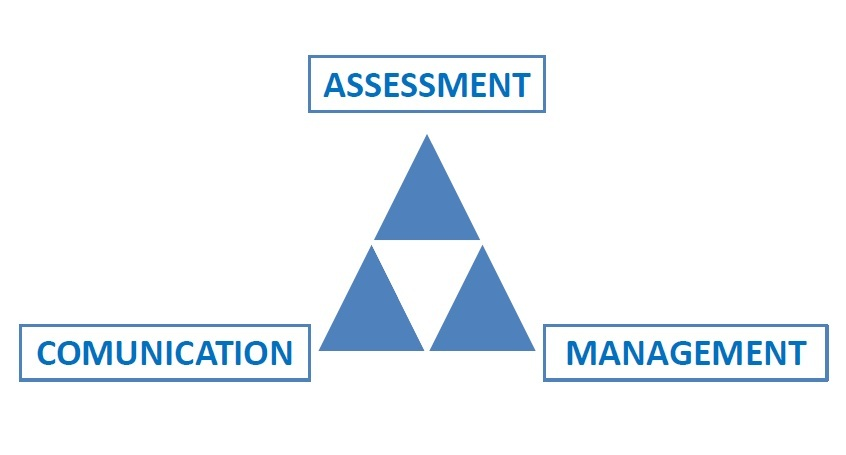
\includegraphics[width=0.5\textwidth]{26/image2.jpeg}
	\end{figure}

\textbf{Assessment} (Valutazione), \textbf{Management} (Gestione) e
\textbf{Comunicazione}, in quest'ordine.

\subsubsection{Assessment (valutazione)}

Cosa rientra nella valutazione?

\begin{itemize}
\item
  \textbf{Riconoscere l'emergenza:} innanzitutto è necessario
  riconoscere che si è di fronte ad un'emergenza (in alcuni casi
  eclatante, in altri casi è necessario un meccanismo di allerta che
  permetta di riconoscere tempestivamente che si tratti di
  un'emergenza);
\item
  \textbf{Quantificare i danni ed i possibili danni} se l'emergenza non
  viene contenuta ed evitata;
\item
  \textbf{Identificare i bisogni della popolazione colpita} \textbf{ma
  anche della popolazione a rischio;}
\item
  \textbf{Pianificare ed implementare la fase successiva di gestione.}
\end{itemize}

In una prospettiva più ampia, i dati raccolti in una condizione di
emergenza sanitaria vengono utilizzati per:

\begin{itemize}
\item
  \textbf{Comunicazione tra i diversi settori coinvolti}, al fine di
  facilitare un'azione che è coordinata tra i vari attori;
\item
  \textbf{Informazione pubblica} che sia veritiera;
\item
  \textbf{Ai fini di un'''Advocacy''} a livello finanziario-politico
  (\emph{``advocacy''}: supportare una causa, richiedere dei fondi,
  richiedere che un certo argomento sia messo nell'agenda politica di un
  paese, di una regione, di una nazione). Il supporto dei dati aumenta
  le probabilità di ottenere buoni risultati.
\end{itemize}

L'intero filone dell'epidemiologia delle emergenze e dei sistemi di
sorveglianza è una branca molto importante della sanità pubblica anche a
livello territoriale. Per cui \emph{``assessment''} periodici per la
valutazione ed il monitoraggio della risposta all'emergenza sono
rilevanti.

Per approfondimenti, la scuola John Hopkins di Baltimora, una delle
scuole di sanità pubblica più famose al mondo, ha un'intera sezione
dedicata ai principi di base dell'epidemiologia delle emergenze (ad
esempio come fare un'analisi quantitativa, quindi una valutazione in
casi di emergenza sanitaria, ai fini di programmare in maniera ottimale
la fase di gestione). Materiale utile presente anche sui siti del CDC.

\begin{figure}[!ht]
\centering
	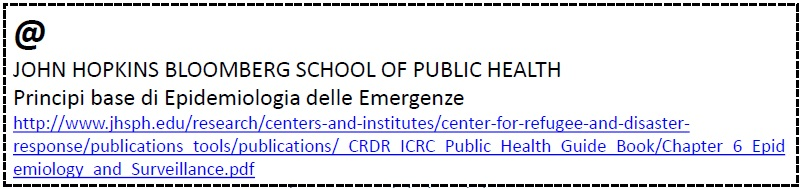
\includegraphics[width=0.5\textwidth]{26/image3.jpeg}
	\end{figure}

Una volta che è stata terminata la valutazione si passa alla fase
successiva di gestione.

\subsubsection{Management (gestione)}

Qui ritorna il concetto di \emph{preparedness}. La gestione parte, ed è
tanto più di successo, quando c'è un sistema, definito in condizioni di
non emergenza, pianificato per rispondere all'emergenza stessa.
Ulteriore definizione di \emph{preparedness} è la capacità di prevenire
e di rispondere alle condizioni di emergenza sanitarie. Tutto questo è
molto teorico e funzionante, ma tutto sta nell'applicarlo alle diverse
condizioni di emergenza sanitaria presenti nella lista sopra menzionata.

La \textbf{gestione} delle emergenze sanitarie comprende tutte le azioni
volte a:

\begin{itemize}
\item
  \textbf{Evitare} (\emph{prevention})
\item
  \textbf{Contenere} gli effetti negativi di un'emergenza sanitaria già
  in atto (\emph{mitigation \& preparedness})
\end{itemize}

\subsubsection{Comunicazione}

L'aspetto comunicativo, in ambito di sanità pubblica ed a maggior
ragione in condizioni di emergenza sanitaria, è di fondamentale
importanza nella gestione delle emergenze soprattutto perché le
conseguenze di un'errata comunicazione possono peggiorare la gestione
dell'emergenza. Ad esempio: le persone a rischio, ovvero non colpite,
dovrebbero adottare dei comportamenti tesi a diminuire l'impatto
dell'emergenza. Se, a causa di comunicazioni errate, si comportassero in
maniera errata andrebbero a peggiorare la gestione dell'emergenza. È
quindi opportuno ricercare dov'è la responsabilità di una comunicazione
corretta in una condizione di emergenza sanitaria.

Questo partendo dall'assioma di base secondo cui l'esistenza e l'entità
di un rischio molto spesso non sono correlate con le reazioni della
popolazione: la percezione del rischio non è direttamente correlata
all'entità del rischio stesso. Le reazioni della popolazione sono per la
maggior parte indotte dalle forme comunicative con cui i rischi o le
emergenze vengono presentati.

Le reazioni della popolazione influiscono sull'evoluzione e sull'esito
delle situazioni di emergenza, in quanto un disorientamento può
compromettere la necessaria collaborazione in azioni di sanità pubblica.
Da ciò si deduce come la comunicazione sia un elemento cruciale nella
gestione delle emergenze.

Gli attori coinvolti nei processi comunicativi durante le emergenze
sono:

\begin{itemize}
\item
  \textbf{le istituzioni} (secondo lo slogan americano \emph{«be first,
  be right, be credible, express empathy, promote action, show
  respect»}): l'istituzione deve essere la prima nel dare informazioni,
  devono essere informazioni corrette, sono necessari autorevolezza e
  credibilità nel messaggio trasmesso, deve manifestare una vicinanza
  alle persone colpite o a rischio, promuovere l'azione e dimostrare
  rispetto;
\item
  \textbf{i politici}, i quali non coincidono con le istituzioni in
  quanto molte volte in un discorso politico essi fanno riferimento a
  potenziali elettori quindi alcuni messaggi possono essere
  strumentalizzati;
\item
  \textbf{i tecnici}, spesso carenti da un punto di vista comunicativo;
\item
  \textbf{i giornalisti}, spesso alla ricerca di sensazionalismo.
\end{itemize}

\emph{Riflessione:} Tenendo presente che la comunicazione influisce
pesantemente sul comportamento dei soggetti in condizioni normali ed
ancor più in condizioni di emergenza, come i dati dimostrano, ci si
domanda di chi sia la responsabilità in caso di comunicazione erronea o
fuorviante. Se in un percorso comunicativo ci sono numerose persone
coinvolte (c'è l'istituzione che rilascia la dichiarazione, c'è il
comunicato stampa, c'è il giornalista che interpreta il comunicato e
scrive l'articolo o fa un video) dove sta la responsabilità di fare
giusta comunicazione in ambito sanitario?

Un esempio pratico risale al 2014, quando è stata sollevata l'emergenza
del lotto di vaccino anti influenzale inizialmente associato a morti
sospette in soggetti adulti, ritirato dal mercato in via precauzionale,
poi scagionato dalle indagini di laboratorio. Nel novembre del 2014 il
Corriere della Sera titolava: «Vaccino anti-influenza, quattro morti
sospette». Questo è un esempio in cui la ricerca di sensazionalismo da
parte dei giornalisti fa un'azione controproducente nei confronti di un
messaggio corretto di sanità pubblica e prevenzione. Per approfondimenti
esistono delle fonti americane che danno delle indicazioni su come fare
buona comunicazione in caso di emergenza:

\begin{figure}[!ht]
\centering
	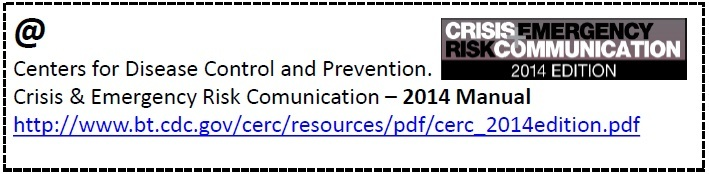
\includegraphics[width=0.5\textwidth]{26/image4.jpeg}
	\end{figure}

\subsection{Gli attori e i livelli}

In generale, quando siamo di fronte ad una emergenza sanitaria, la
gestione prevede il coinvolgimento di più attori e più livelli (nel caso
dell'esempio precedente del terremoto, include il coinvolgimento di
attori a livello \emph{locale/regionale} e \emph{nazionale;} mentre per
altre emergenze, come ad esempio pandemie o emergenze di tipo infettivo,
verrà coinvolto anche il livello \emph{sovranazionale}). Calzanti gli
esempi di Chernobyl, emergenza ambientale ma anche sanitaria che ha
assunto una rilevanza internazionale, e pandemia SARS, emergenza
infettiva recente.

\subsubsection{Dimensione nazionale}

Quali sono i diversi livelli che si occupano di emergenza a livello
italiano?

\begin{itemize}
\item
  A \emph{livello} \emph{territoriale/locale} esistono i
  \emph{dipartimenti di prevenzione delle ASL};
\item
  Esiste un \emph{livello regionale};
\item
  E poi a \emph{livello nazionale} esistono i diversi \emph{Ministeri},
  tra cui il Ministero della Salute ma non solo, e la \emph{Protezione
  Civile}.
\end{itemize}

Nei Livelli Essenziali di Assistenza (\textbf{LEA}) sono garantite le
attività di emergenza sanitaria territoriale e le attività volte alla
predisposizione di sistemi di risposta ad emergenze secondo questo
flusso: Ministero della Salute -> Regioni -> Asl.

Cosa è e di cosa si occupa la Protezione Civile? È parte del servizio
nazionale che coinvolge le amministrazioni ed è costituito da un insieme
di strutture operative che comprendono anche il sistema sanitario
(istituita con legge 24 febbraio 1992 n. 225).

\subsubsection{Dimensione sovranazionale e contesto comunitario}

Perché in alcuni casi i management locali, regionali e nazionali non
sono più sufficienti ma deve entrare in campo la Comunità Europea? Un
esempio su tutti sono le patologie infettive che, secondo meccanismi di
trasmissione propri, non rispettano i confini nazionali diffondendosi in
altri Paesi o Continenti (es. pandemia della SARS).

In generale, il processo di globalizzazione con il trasporto delle
persone, degli animali, dei cibi e di altri prodotti, favorisce il fatto
che i rischi sanitari viaggino in maniera più rapida e questo presuppone
una \emph{preparedness} a livello internazionale.

Viene sottolineato il ruolo che la Commissione Europea può avere nella
risposta alle emergenze: ``l'Europa è messa in una condizione ideale per
coordinare il livello europeo di gestione delle emergenze''.

In ultimo tenere presente che, se alcuni Paesi sono colpiti da una
determinata emergenza sanitaria, le competenze e le risorse di altri
Paesi possono avere un ruolo di supporto.

Tutto questo è sancito dalla normativa europea con il \textbf{Trattato
di Lisbona (art. 168)} e più recentemente nel 2013 la \textbf{Decisione
del Consiglio} della ``cross-border threaths to health'' che riporta
qual è la funzione dell'Europa nella gestione e nella risposta di
possibili emergenze sanitarie.

\begin{figure}[!ht]
\centering
	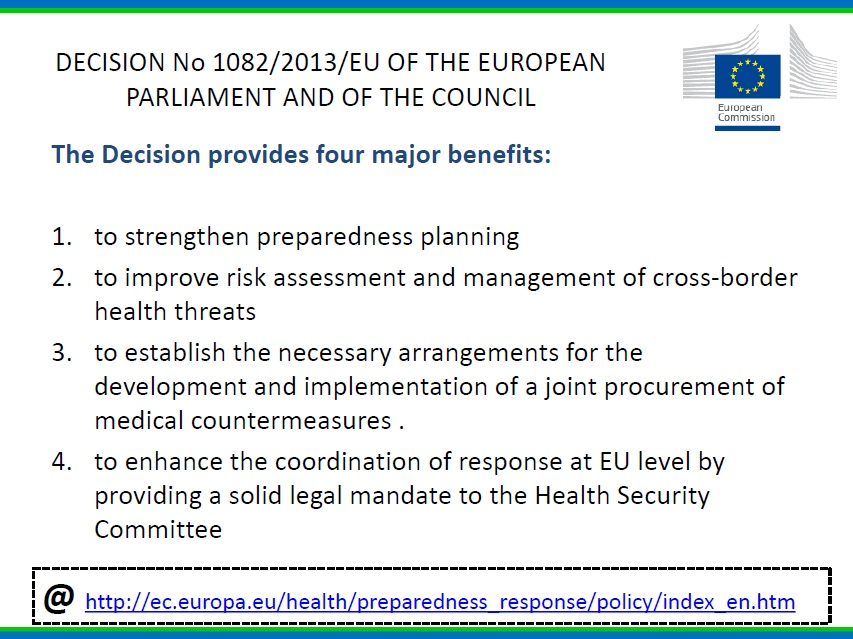
\includegraphics[width=0.5\textwidth]{26/image5.jpeg}
	\end{figure}

\subsubsection{Contesto internazionale (International Health Regulations IHR)}

Qui non parliamo più di Europa, ma di Nazioni Unite e di Organizzazione
Mondiale della Sanità. L' \textbf{International Health Regulations
(IHR)} è un documento, entrato in vigore nel 2007, che stabilisce con
potere di legge quali siano le circostanze nelle quali i Paesi devono
riportare all'OMS alcune emergenze sanitarie di origine infettiva.

Per esempio, se in Italia venisse trovato un caso di poliomielite
naturale o vaccino-indotto, l'Italia sarebbe obbligata a riportare il
caso all'OMS secondo quanto stabilito da questo documento. Si tratta
quindi di uno strumento legale che vincola tutti i Paesi membri delle
Nazioni Unite (196 Paesi) al fine di aiutare la comunità internazionale
a prevenire e rispondere a quei problemi di sanità pubblica che possano
rappresentare una minaccia.

L'OMS informa con un'infografica le ragioni per cui questo strumento è
stato messo a punto (successivamente all'emergenza SARS), per cercare di
fornire uno strumento internazionale di supporto in caso di emergenza
sanitaria.

\begin{figure}[!ht]
\centering
	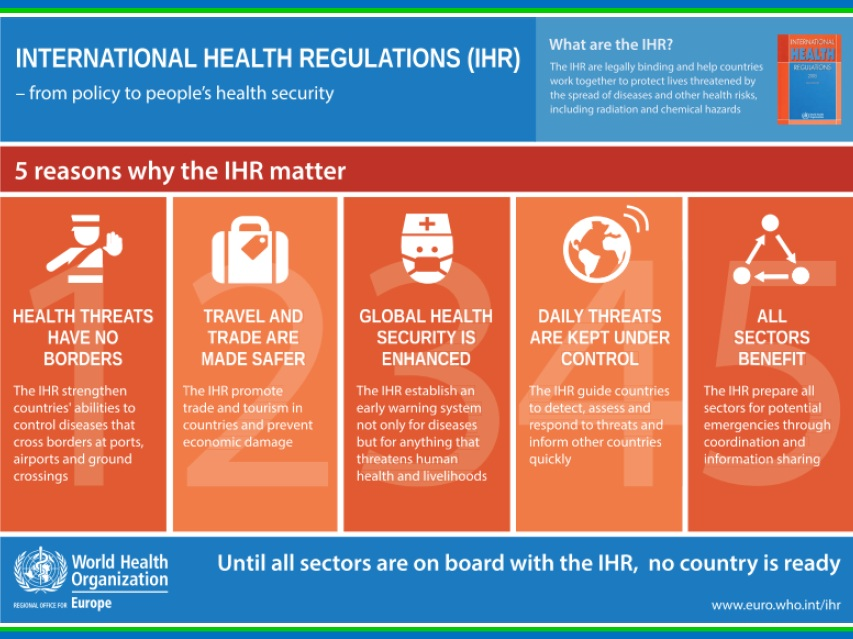
\includegraphics[width=0.5\textwidth]{26/image6.jpeg}
	\end{figure}

\subsection{Epidemie di malattie infettive}

Che cos'è un \textbf{``outbreak''} di malattia infettiva?

\begin{itemize}
\item
  Incidenza di casi di malattia in numero superiore rispetto a quello
  che normalmente ci aspetteremmo secondo i pattern epidemiologici di
  una determinata regione geografica in un determinato periodo
  dell'anno.

Un outbreak può verificarsi sia in una regione geografica specifica
oppure, in base all'agente in questione, estendersi anche in diversi
Paesi. Inoltre, in base al tipo di microrganismo, può avere una durata
di alcuni giorni, alcune settimane o anche diversi anni.

\item
  Un singolo caso di malattia infettiva che non si era mai verificato o
  non si verificava da tempo in una determinata area, rientra nella
  definizione di outbreak.
  
\end{itemize}

``In definitiva intendiamo per outbreak un'occorrenza di casi lì dove
non ce li aspettiamo''.

Le agenzie sanitarie, in questo caso l'ECDC (corrispettivo europeo del
CDC) spiegano cosa fare per condurre un'indagine epidemiologica in caso
di outbreak.

\begin{figure}[!ht]
\centering
	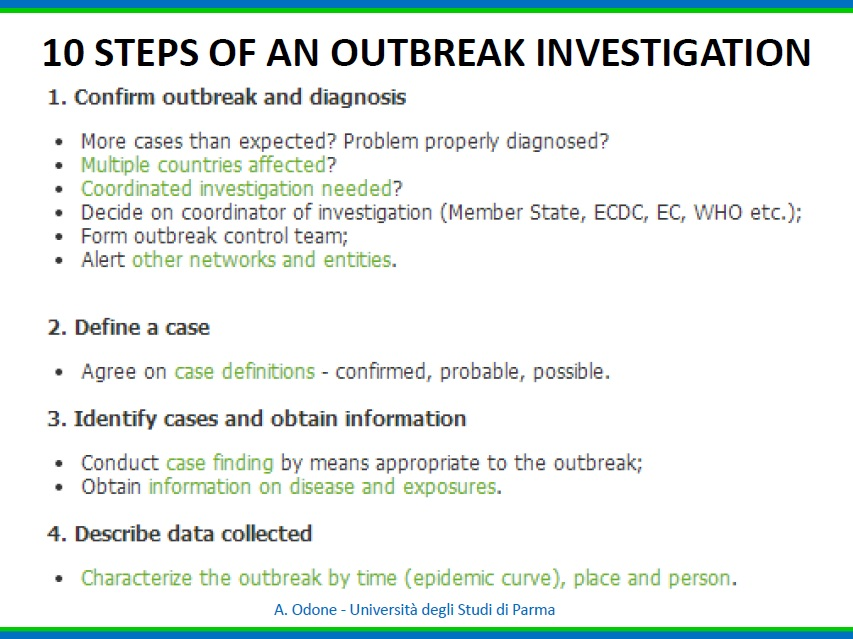
\includegraphics[width=0.5\textwidth]{26/image7.jpeg}
	\end{figure}
	
\begin{figure}[!ht]
\centering
	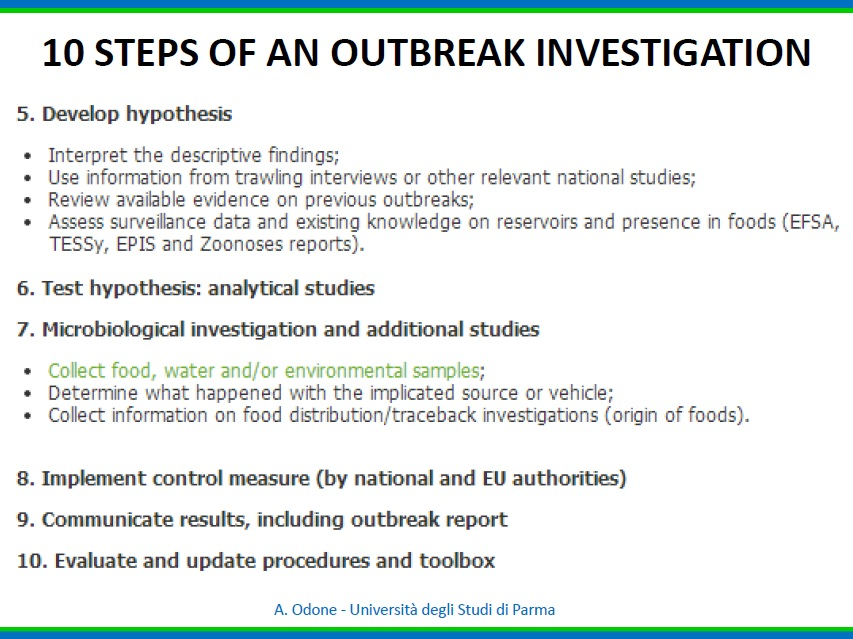
\includegraphics[width=0.5\textwidth]{26/image8.jpeg}
	\end{figure}

Innanzitutto, secondo la triangolazione vista in precedenza, bisogna
riconoscere un outbreak di malattia, cioè confermare il fatto che ci sia
un outbreak ed individuare il microrganismo in questione.
\\\\
\textbf{Step 1:} \textbf{confermare l'outbreak e fare diagnosi}. Come ci
si arriva? Inizialmente dall'\emph{osservazione} \emph{empirica} che ci
sono più casi rispetto a quelli che ci aspetteremmo. Poi è necessaria
una valutazione di \emph{quanti} Paesi sono coinvolti ed in base a
quello decidere la \emph{risposta} ed il \emph{management}. Gli altri
step sono molto specifici per un operatore della sanità pubblica.
\\\\
\textbf{Step 2:} \textbf{definire un caso} catalogandolo tra i
\emph{sospetti, possibili, probabili e confermati}.
\\\\
Una volta che è stato identificato e definito il caso, è opportuno:

\begin{itemize}
\item
  identificare i casi nel contesto di riferimento e raccogliere i dati;
\item
  sviluppare un'ipotesi di origine del caso;
\item
  fare tutte le indagini di laboratorio per identificare il
  microorganismo e capire la sorgente di infezione;
\item
  implementare misure di controllo;
\item
  comunicare i risultati ai vari livelli e mettere tutto quello che si è
  immagazzinato a livello di dati, esperienza e controllo a disposizione
  di una futura emergenza (\emph{preparedness}).
\end{itemize}

Come riconoscere una curva epidemiologica in caso di outbreak. Esempio
tratto da una descrizione pubblicata sul New England del 2011 di
Sindrome Emolitico-uremica in Germania.

\begin{figure}[!ht]
\centering
	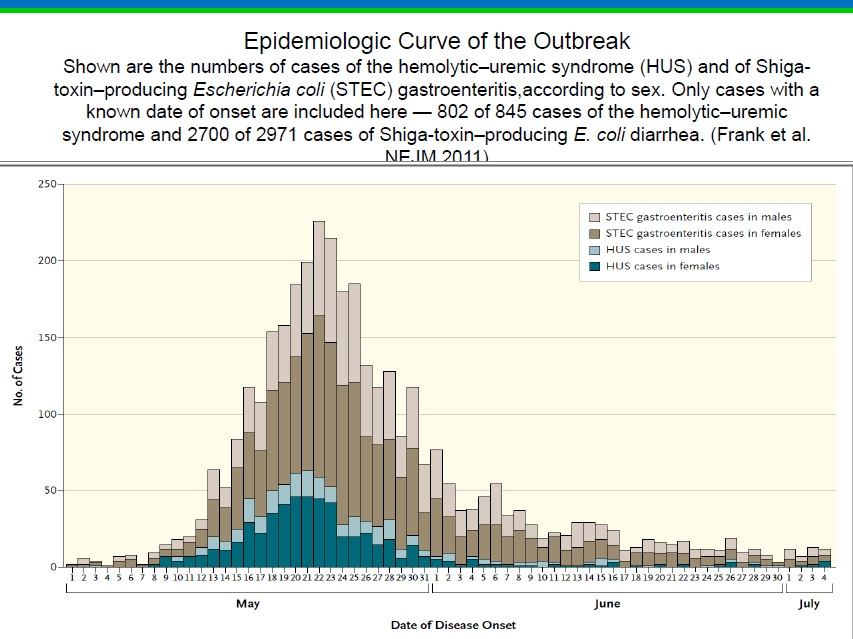
\includegraphics[width=0.5\textwidth]{26/image9.jpeg}
	\end{figure}

Nell'eventualità di un outbreak, i casi vengono collocati su un piano
cartesiano, dove vengono messi in ordinata il numero di casi ed in
ascissa il tempo in cui si sviluppano e vengono diagnosticati. La forma
della curva epidemiologica (fatte dall'igiene pubblica, dagli
epidemiologi) permette di avere delle indicazioni sul microrganismo in
oggetto, in quanto molte volte potrebbe non essere ancora stato
identificato (es. la temporalità da indicazioni sul tempo di
incubazione, il numero di casi contagiati da informazioni sulla
virulenza) conseguentemente quali sono le misure di controllo da
adottare per contenere l'ulteriore trasmissione dell'infezione.

Ecco alcuni grandi esempi di epidemie di malattie infettive a cui si è
dovuto far fronte anche con una gestione a livello internazionale nelle
decadi passate:

\begin{itemize}
\item
  la \textbf{SARS}, emersa in Cina nel 2003 e rapidamente trasmessa al
  Canada (caso eclatante che a livello aneddotico offre numerosi spunti
  su cui studiare gli outbreak di malattia);
\item
  la \textbf{pandemia influenzale H1N1} più recente;
\item
  l'\textbf{ebola,} di cui il CDC riportava dei dati raccolti ai fini di
  assessment, quali la numerosità dei casi e delle morti d'ebola
  suddivise per Paese, slot temporale e per definizione di caso
  (confermato, probabile, sospetto). Sul sito del CDC (ma anche su
  quello del ECDC anche se meno aggiornato) si possono leggere in tempo
  reale i bollettini di sorveglianza dell'ebola e di altre patologie a
  rischio di emergenza sanitaria.
\end{itemize}

\subsection{Medicina delle emigrazioni ed emergenza migranti}

Se parliamo in generale di Medicina delle emigrazioni dobbiamo tener
conto di alcuni pattern demografici che caratterizzano un Paese; per
esempio l'Italia è considerato un Paese di recente immigrazione, nel
senso che è stato per decenni un Paese da cui la gente emigrava e solo
da due generazioni è un Paese che accoglie i migranti.

\begin{figure}[!ht]
\centering
	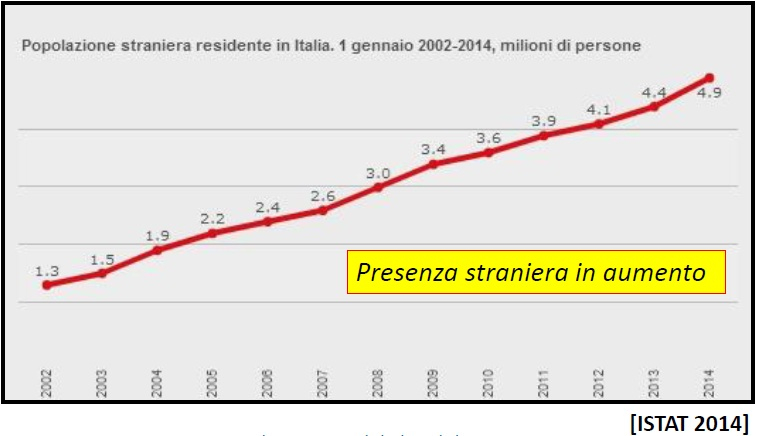
\includegraphics[width=0.5\textwidth]{26/image10.jpeg}
	\end{figure}

Secondo l'ISTAT, il numero di persone straniere residenti in Italia ha
superato i 5 milioni, con un trend in aumento.

\begin{figure}[!ht]
\centering
	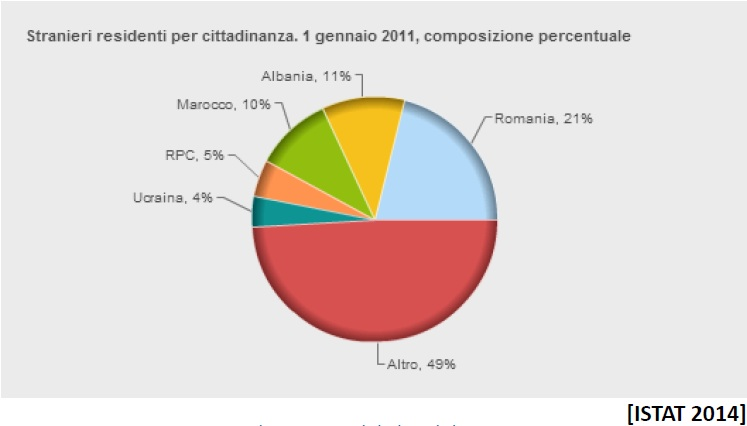
\includegraphics[width=0.5\textwidth]{26/image11.jpeg}
	\end{figure}

Questi sono i Paesi di origine della popolazione straniera presente in
Italia. Sono grafici specifici per ogni Paese ospite e variano molto tra
loro, per una questione di rotte, di tradizione culturale, ecc.

\begin{figure}[!ht]
\centering
	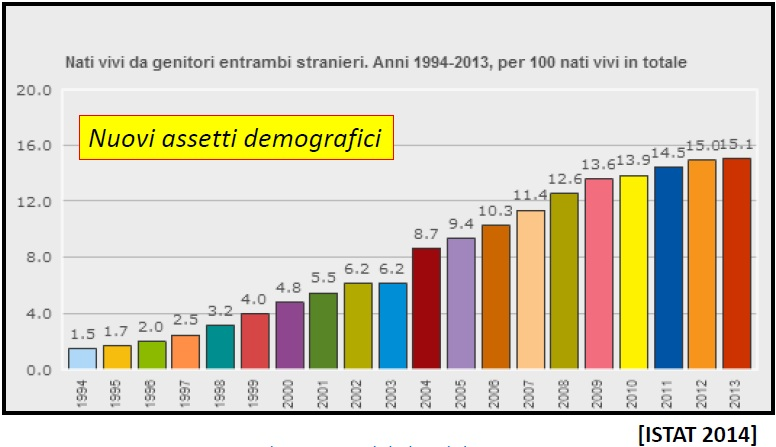
\includegraphics[width=0.5\textwidth]{26/image12.jpeg}
	\end{figure}

Non solo la presenza straniera è in aumento ma ci sono nuovi
\emph{assetti demografici}. Ad esempio, questi sono i nuovi nati vivi da
entrambi i genitori stranieri e non classificati dall'ISTAT come
immigrati ma come italiani (dal momento che la suddivisione statistica
viene fatta in base al Paese di nascita, essi ``sfuggono'' alle
statistiche).

\begin{figure}[!ht]
\centering
	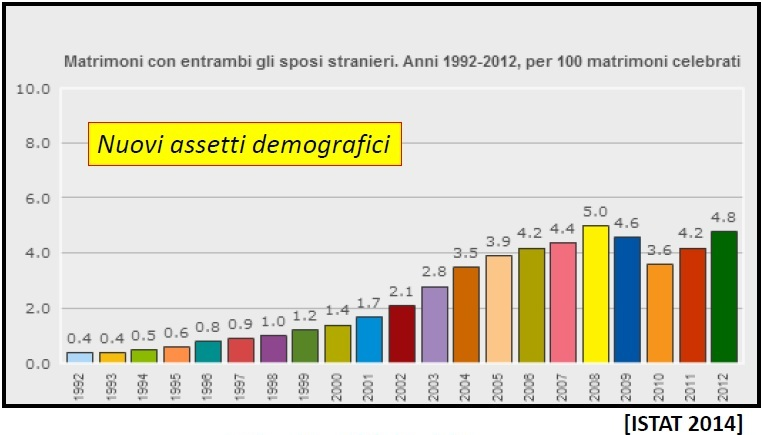
\includegraphics[width=0.5\textwidth]{26/image13.jpeg}
	\end{figure}

Questi sono i matrimoni contratti in Italia con entrambi gli sposi
stranieri a sottolineare come, dati alla mano, la popolazione di origine
straniera si stia progressivamente integrando nella comunità del nostro
Paese.

\begin{figure}[!ht]
\centering
	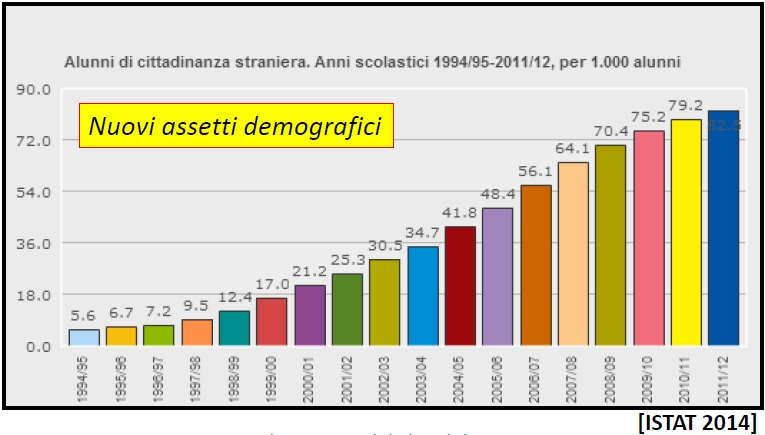
\includegraphics[width=0.5\textwidth]{26/image14.jpeg}
	\end{figure}

Un altro esempio sono gli alunni con cittadinanza straniera e così via.

Tutti i dati sono disponibili sul sito dell'ISTAT con dei report
particolarmente interessanti ed approfonditi sui migranti.

\begin{figure}[!ht]
\centering
	
\includegraphics[width=0.5\textwidth]{26/image15.jpeg}
	\end{figure}

Nell'organizzazione dello studio della medicina della migrazione, è
opportuno partire da una suddivisione.

\begin{itemize}
\item
  \textbf{Fase acuta} all'interno della quale rientrano le emergenze
  socio-sanitarie legate all'arrivo dei migranti;
\item
  \textbf{Fase cronica}, definita tale per ragioni didattiche, ovvero
  problematiche socio-sanitarie della popolazione migrata residente (es.
  diversa distribuzione dei fattori di rischio, dell'accesso alle cure,
  ecc.).
\end{itemize}

Si è parlato moltissimo su giornali nazionali ed internazionali
dell'emergenza socio-sanitaria legata allo sbarco di migranti. Al di là
della personale percezione della questione, si tratta sicuramente di una
problematica politica, umana e sanitaria che ha raggiunto dimensioni
rilevanti soprattutto negli ultimi anni e soprattutto per il Paese
italiano che tra quelli europei è tra i maggiormente interessati.
L'Italia per la sua posizione geografica è considerata porta d'Europa
quindi l'afflusso è consistente, soprattutto via mare, dal Nord Africa e
dall'Europa dell'Est.

La tragedia di Lampedusa, probabilmente la più tristemente nota, è stata
il ``trigger'' che ha spinto il Ministero dell'Interno ad organizzare
l'operazione ``Mare Nostrum'', successivamente fatta propria
dall'Europa. Iniziata nel 2014, è definita come un'operazione militare e
umanitaria attuata dalle Forze della Marina e dell'Aeronautica Militare
Italiane nel mar Mediterraneo meridionale, nata per fronteggiare lo
stato di emergenza umanitaria in corso nello stretto di Sicilia, quindi
per garantire la salvaguardia della vita in mare ed assicurare alla
giustizia tutti coloro i quali lucrano sul traffico illegale di
migranti. Questa operazione includeva una componente della gestione
dell'emergenza sanitaria della popolazione in sbarco.

Quali possono essere gli aspetti sanitari che devono essere presi in
considerazione nella gestione di questo tipo di emergenza?

Le condizioni di viaggio sono condizioni di sovraffollamento, quindi
dovranno essere ricercate patologie con trasmissione aerea, esposizione
a carenze alimentari, avvelenamento, intossicazione.

La condizione di endemia di alcune patologie nel Paese di origine può
essere un rischio per la popolazione dei residenti del Paese ospitante,
ma in realtà, seppur si tratti di un rischio teoricamente plausibile, i
dati dimostrano che la trasmissione di alcune patologie, come ad esempio
la tubercolosi che può essere endemica nei Paesi d'origine, non è una
problematica rilevante di sanità pubblica per diversi motivi (ad esempio
perché alcune patologie come la tubercolosi si trasmettono con contatto
diretto ed ancora le comunità straniere sono separate dalle comunità
italiane). Questo rischio, cavalcato in maniera strumentale in alcuni
contesti, non è una rilevante problematica in ambito di salute pubblica.

Ulteriori fattori di rischio a cui sono esposti i migranti durante il
viaggio in condizioni disagevoli, oltre al rischio infettivo, sono i
rischi legati ad infortuni (in cui includiamo anche naufragi, ecc).

\begin{figure}[!ht]
\centering
	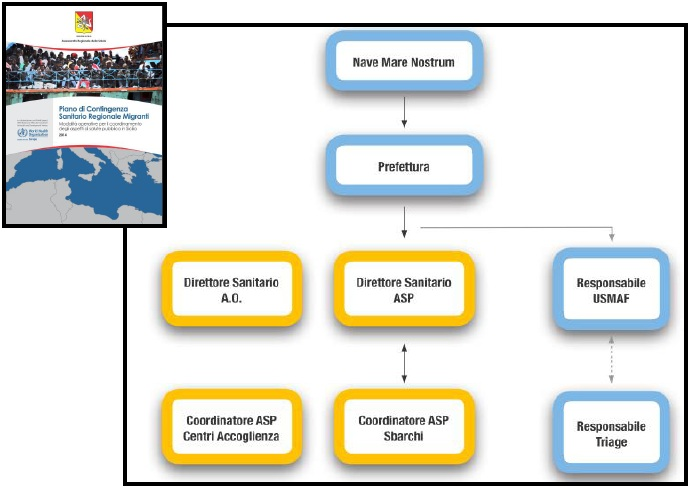
\includegraphics[width=0.5\textwidth]{26/image16.jpeg}
	\end{figure}
	
Tutto questo per evidenziare come siano stati organizzati piani di
contingenza specifici da parte delle Regioni e delle AUSL per la
gestione del rischio sanitario. Nell'immagine è schematizzato il piano
adottato dalla Regione Sicilia, sicuramente tra quelle che hanno dovuto
maggiormente far fronte in questi ultimi anni all'emergenza migranti.
Secondo tale schema, venivano attribuite alle singole autorità
competenti differenti mansioni nella gestione dell'emergenza sanitaria,
distribuite tra ASL, Sanità Territoriale e Forze dell'Ordine e
Prefettura.

I rischi per la salute vengono suddivisi in tre categorie:

\begin{itemize}
\item
  Rischi relativi al viaggio (journey);
\item
  Rischi connessi con le operazioni di soccorso in mare e lo sbarco;
\item
  Rischi relativi alla permanenza nei centri di prima accoglienza
  (luoghi in cui i rischi per la salute sono più alti rispetto ai rischi
  della popolazione generale).
\end{itemize}

L'Emilia Romagna, come tutte le Regioni italiane, è stata coinvolta nel
programma di smistamento della popolazione migrante (anche senza
documenti) sul territorio italiano. Tramite una circolare indirizzata ai
Direttori Generali, territoriali AUSL ed ospedalieri, sono state
diramate le direttive omogenee per l'assistenza sanitaria alle persone
straniere all'interno del programma italiano Mare Nostrum. Allegata alla
circolare, una checklist prevede quali siano gli esami diagnostici da
effettuare dai medici a livello locale e territoriale per fare un
assessment delle persone smistate nei territori della regione.

Quali sono gli accertamenti che il medico territoriale deve fare in una
persona che si presenta non perché malata ma perché semplicemente
migrante di recente arrivo, tenendo presente i rischi di questa
popolazione?

\begin{itemize}
\item[1.]  
  La checklist della prima visita prevede la raccolta dei dati personali
  (da specificare la lingua parlata e l'eventuale necessità di un
  interprete) e dei dati concernenti il viaggio, il Paese di origine
  (per avere una visione d'insieme sulle endemie del Paese di origine)
  eventuali Paesi attraversati (molto spesso il percorso migratorio è
  molto lungo) e relativi tempi di permanenza; specificare se sia stata
  effettuata un'assistenza sanitaria allo sbarco; effettuare un'anamnesi
  patologica remota, volta ad identificare la presenza di pregresse
  esposizioni a fattori di rischio ed un'anamnesi patologica prossima,
  inclusa una valutazione circa un eventuale stato di gravidanza;
  l'esame obiettivo è focalizzato soprattutto sulla ricerca di problemi
  di tipo dermatologico e respiratorio (proprio perché un soggetto che
  ha appena compiuto un viaggio può essere sottoposto a rischio
  infettivo di alcune patologie a trasmissione aerea o cutanea) e su
  altre valutazioni come quella delle stazioni linfonodali, valutazioni
  cardiologica, intestinale, odontoiatrica ecc.
\item[2.]
  Screening per la tubercolosi e vaccinazioni, in una fase successiva di
  prevenzione e profilassi da attuare nelle sedi di accoglienza
  territoriale.
\end{itemize}

Quali potrebbero essere i problemi legati all'effettuazione di queste
valutazioni, contenute nel protocollo a livello nazionale, in maniera
corretta ed omogenea? Si annoverano la collaborazione dei soggetti,
condizionata da fattori come lingua, aspetti culturali, aspetti
religiosi, oltre alla difficoltà di uniformare la scheda vaccinale e
risalire alle vaccinazioni pregresse fatte nella popolazione adulta.

Verrà affrontata successivamente la parte riguardante la fase cronica
sulle popolazioni immigrate non recentemente arrivate. Si tratta di
popolazioni straniere che vivono in Italia e che presentano una serie di
fattori di rischio ed un accesso alle cure che possono essere differenti
rispetto a quelle della popolazione italiana e che quindi meritano degli
approfondimenti.

Tra le emergenze sanitarie annoveriamo anche le catastrofi che fanno
riferimento a situazioni quali il terrorismo o catastrofi naturali come
terremoti, alluvioni, tsunami ecc, di cui abbiamo portato alcuni esempi.

Un'applicazione del concetto di \emph{preparedness} in Emilia Romagna,
potrebbe essere ad esempio avere a disposizione degli opuscoli pronti
che possono guidare la popolazione sui comportamenti da avere, numeri di
emergenza e azioni da fare in caso di terremoto. Questo difatti è uno
strumento della \emph{preparedness}, in quanto l'assessorato dell'Emilia
Romagna redige questo opuscolo che sarà reso disponibile nel momento di
emergenza sanitaria.